\label{chap:evaluation}

In this chapter we evaluate various aspects of our work in structure detection.
We first present a technical evaluation of the algorithm, assessing the quality of its output and runtime performance. We also look at the performance characteristics achieved when incorporating our structure detection into the core-computation work-flow.


\section{Benchmarks}
We briefly introduce the sample meshes used as benchmarks.

\subsection{Airfoil grid mesh}
This is a mesh generated using the \texttt{naca0012.m} script~\cite{airfoilgen}, following the NACA0012 definition for constructing an airfoil upper surface. It is parametrised by two variables $I$ and $J$ which denote the length and width of the airfoil boundary. The default airfoil mesh size is is built with $I=400$ and $J=600$, containing about 720,000 vertices. Topologically, the vast majority of the mesh forms a single large rectangular structure. Figure~\ref{fig:airfoil-mesh} shows a sample rendering.

\begin{figure}
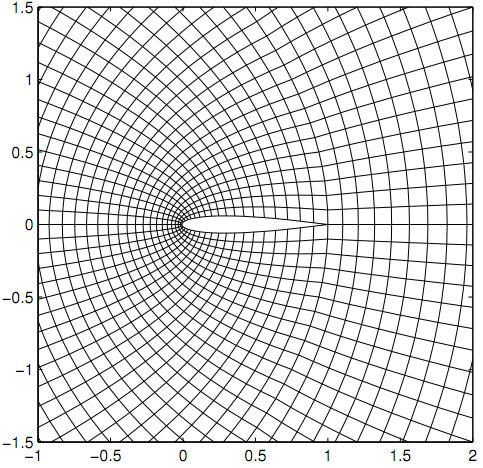
\includegraphics[width=\textwidth]{images/evaluation/airfoil.jpeg}
\caption{A rendering of a small sample of the airfoil mesh generated by~\cite{airfoilgen}. The image was obtained from \cite{Tkachov2012thesis}.}
\label{fig:airfoil-mesh}
\end{figure}

\subsection{NACA0012 mesh}
This mesh was generated from \texttt{naca0012.geo}, kindly provided by George Ntemos, using Gmsh~\cite{geuzaine2008gmsh}. It represents the construction of a NACA0012 airfoil at zero incidence. The mesh is fairly coarse, containing roughly 15,000 vertices. Figure~\ref{fig:naca0012-mesh} shows sample renderings.

\begin{figure}
\sidebysidevertical
{
  \includegraphics[width=\textwidth]{images/evaluation/naca0012.pdf}
  \caption{A wide shot of the airfoil.}
}
{
  \includegraphics[width=\textwidth]{images/evaluation/naca0012-closeup.pdf}
  \caption{A close-up at the airfoil border. Note the highly structured region formed directly around the airfoil.}
}
\caption{A rendering of the naca0012 airfoil mesh.}
\label{fig:naca0012-mesh}
\end{figure}

\subsection{NACA0021 mesh}
This mesh was generated from \texttt{naca0021.geo}, kindly provided by Harry Davis, using Gmsh~\cite{geuzaine2008gmsh}. It represents the construction of a NACA0021 airfoil at a 60 degree angle of attack. The mesh contains roughly 20,000 vertices. Figure~\ref{fig:naca0021-mesh} shows sample renderings.

\begin{figure}
\sidebysidevertical
{
  \includegraphics[width=\textwidth]{images/evaluation/naca0021.pdf}
  \caption{A (very) wide shot of the airfoil. The diagonal facing spec in the middle is the airfoil!}
}
{
  \includegraphics[width=\textwidth]{images/evaluation/naca0021-closeup.pdf}
  \caption{A close-up at the airfoil border. Note the large structured region formed behind the airfoil.}
}
\caption{A rendering of the naca0021 airfoil mesh.}
\label{fig:naca0021-mesh}
\end{figure}


\subsection{The airfoil computation}
\label{subsec:airfoil-computation}
The airfoil computation is an example core-computation which is used as an example application in OP2~\cite{op2airfoil}. The computation applies the volume method to solve the 2D Euler equations iteratively, refining the solution until a steady state is reached. Within each iterations it performs multiple loops over cells and meshes, which involve both reading and writing data.

This application serves as a good benchmark, as it allows us to
\begin{enumerate*}[label=\alph*)]
\item compare our performance against OP2's, and
\item compare out computed results against OP2's, to ensure correctness.
\end{enumerate*}

\section{Metrics}
\subsection{Core-computation metrics}
There are three types of core-computation executions which we evaluate:
\begin{itemize}
\item Baseline OP2 execution time
The runtime of the core-computation with OP2~\cite{op2common}, which does not use any structured region information. Mesh elements are accessed using indirection maps.

\item Crystal execution time
The runtime of the core-computation with Crystal using structured region information. Mesh elements in structured regions are accessed directly using address calculations; mesh elements in unstructured regions are accessed using indirection maps.

\item Unstructured Crystal execution time
The runtime of the core-computation with Crystal \emph{without} providing structured region information. Mesh elements are accessed using indirection maps. The structured loops are still present in the code, though they are skipped at runtime due to missing structured region information. In effect, this is a competing implementation of the same iteration algorithm used by OP2.
\end{itemize}
All execution measurements exclude initialization and cleaning up time, which in any case have been found to be negligible.

\subsection{Detection metrics}
\begin{itemize}
\item Structured region size:

This is the number of vertices found in a particular structured region. The general notion may refer to the average of such number.
\item Number of structured regions detected
\item Detection coverage: Either the number or percentage (as defined in context) of vertices in the mesh detected as structured elements.
\end{itemize}


\section{Structure detection}
The first step in evaluating our structure detection algorithms, manifested through our implementation, is to answer the simple question: does it work? Using detection metric here is useful, but at a fundamental level the best way to assess whether the implementation works as expected is to visualise the result.


\subsection{Airfoil grid}
Our first structure detection run is performed on the airfoil grid, as it is the simplest case for which we can assess correctness. Figure~\ref{fig:airfoil-grid-visual} shows the result of running structure detection on a very small version of the airfoil grid mesh. We can clearly see that the structured regions are as we would expect, forming a two-dimensional lattice which spans to include all structured vertices.

\begin{figure}
\includesvg[width=\textwidth, svgpath=images/evaluation/]{airfoil_structure}
\caption[Visualisation of detected structure in the airfoil grid mesh]{A rudimentary visualisation\footnotemark{} of the detected structure in an airfoil grid mesh. The mesh is parametrised with $I=4$ and $J=6$, resulting in 91 vertices. Structured vertices and cells are denoting in bright and dull red, respectively. Note that the numbering shown denotes the old mesh numbering.}
\label{fig:airfoil-grid-visual}
\end{figure}\nopagebreak\footnotetext{The custom \texttt{*.dat} used by the authors of this mesh does not make it amenable to visualisation by popular tools. This image was generated using a Python script outputting a graph description, with suitable colour and label information, which is then passed to the \texttt{dot}~\cite{ellson2002graphviz} utility to visualize.}



\subsection{NACA0012}
We now consider more complex meshes where more interesting patterns of structure can be found. First, we detect the structure in the NACA0012 mesh, depicted in figure~\ref{fig:naca0012-structure}. Notice how the highly structured region surrounding the borders of the airfoil is cleanly detected as one big structured region. However, looking at the small patches of structure, it is clear that there have been some losses. All these losses, however, are distinctly attributable to our choice of length-first search, which we described in subsection~\ref{subsec:length-first-search} as being eager. We shall see an example of this shortly.

Figure~\ref{fig:plot-naca0012-region-sizes} shows the structured region frequency for the NACA0012, averaged over 200 runs. As would be intuitively expected, a small number of large structured regions are discovered, whereas small structured regions are abundant. Structured region size seems to follow a skewed normal distribution, with a peak value at 12.

Figure~\ref{fig:plot-naca0012-node-region-sizes} on the other hand plots the frequency of vertices \emph{belonging to} a structure of a given size. For example, if we partition a mesh into five regions of size 10 and one region of size 100, respectively, then 50 vertices in the mesh belong to a region of size 10, and 100 vertices belong to a region of size 100. Notice how the sizes of structured regions follow a bimodal distribution: they are typically either very small or very large.

\begin{figure}
\sidebysidevertical{
\includegraphics[width=\textwidth]{images/evaluation/naca0012-structure-cropped.pdf}
}
{
\includegraphics[width=\textwidth]{images/evaluation/naca0012-structure-closeup-cropped.pdf}
}
\caption{A visualisation of the detected structure in the NACA0012 mesh.}
\label{fig:naca0012-structure}
\end{figure}


\begin{figure}
\sidebysidevertical
{
\begin{tikzpicture}
  \begin{axis}[
    ybar,
    bar width=0.5mm,
    width=12cm,
    height=5cm,
    % enlarge y limits=0.5,
    xlabel = Structured region size,
	ylabel = Average frequency,
	xmode = log,
    % nodes near coords, nodes near coords align={horizontal},
	legend pos = north west,
    ]
 pos = south east
]


\addplot [
fill=blue!80!white,
% pattern=horizontal lines light blue
] table [
y = frequency,
x = regionsize
] {data-naca0012-region-sizes.tsv};


\end{axis}
\end{tikzpicture}

\caption{Plot of the distribution of structured region sizes.}
\label{fig:plot-naca0012-region-sizes}
}
{
\begin{tikzpicture}
  \begin{axis}[
    ybar,
    bar width=0.5mm,
    width=12cm,
    height=5cm,
    % enlarge y limits=0.5,
    xlabel = Structured region size,
	ylabel = {Vertices in structured regions of the given size},
	xmode = log,
    % nodes near coords, nodes near coords align={horizontal},
	legend pos = north west,
    ]
 pos = south east
]


\addplot [
fill=blue!80!white,
% pattern=horizontal lines light blue
] table [
y expr = \thisrow{frequency} * \thisrow{regionsize},
x = regionsize
] {data-naca0012-region-sizes.tsv};


\end{axis}
\end{tikzpicture}

\caption{Plot of the distribution of structured region sizes to which vertices belong.}
\label{fig:plot-naca0012-node-region-sizes}
}
\caption{Statistics related to the structured region sizes of the NACA0012 mesh.}
\end{figure}




\subsection{NACA0021}
Next we look at the results of structure detection for the NACA0021 mesh, shown in figure~\ref{fig:naca0021-structure}. Interestingly the algorithm failed to detect the obvious targets as a single large chunk, and has instead fragmented it into a few relatively large blocks. Examining the boundaries of this large chunk, we find that it has many ``traps'', that is small portions where an eager structure detection algorithm may extend beyond where its supposed, and then get stuck in a sub-optimal configuration. Figure~\ref{fig:naca0021-good-structure} shows the detected structure when we hand-pick a seed vertex which does not fall into such a ``trap''.





Figure~\ref{fig:plot-naca0021-region-sizes} shows the structured region frequency for the NACA0021, averaged over 200 runs. The results are similar to the NACA0012 results in figure~\ref{fig:plot-naca0012-region-sizes}, and in fact the same peak value of 12 is present here.

Figure~\ref{fig:plot-naca0021-node-region-sizes} shows the frequency of vertices \emph{belonging to} a structure of a given size. It is also similar to the corresponding plot for NACA0012 in figure~\ref{fig:plot-naca0012-node-region-sizes}.


\begin{figure}
\sidebysidevertical{
\includegraphics[width=\textwidth]{images/evaluation/naca0021-structure-cropped.pdf}
}
{
\includegraphics[width=\textwidth]{images/evaluation/naca0021-structure-closeup-cropped.pdf}
}
\caption{A visualisation of the detected structure in the NACA0021 mesh.}
\label{fig:naca0021-structure}
\end{figure}


\begin{figure}
\includegraphics[width=\textwidth]{images/evaluation/naca0021-good-structure-cropped.pdf}
\caption{A visualisation of the detected structure in the NACA0021 mesh when hand-picking a ``good'' seed vertex.}
\label{fig:naca0021-good-structure}
\end{figure}


\begin{figure}
\sidebysidevertical
{
\begin{tikzpicture}
  \begin{axis}[
    ybar,
    bar width=0.5mm,
    width=12cm,
    height=5cm,
    % enlarge y limits=0.5,
    xlabel = Structured region size,
	ylabel = Average frequency,
	xmode = log,
    % nodes near coords, nodes near coords align={horizontal},
	legend pos = north west,
    ]
 pos = south east
]


\addplot [
fill=blue!80!white,
% pattern=horizontal lines light blue
] table [
y = frequency,
x = regionsize
] {data-naca0012-region-sizes.tsv};


\end{axis}
\end{tikzpicture}

\caption{Plot of the distribution of structured region sizes.}
\label{fig:plot-naca0021-region-sizes}
}
{
\begin{tikzpicture}
  \begin{axis}[
    ybar,
    bar width=0.5mm,
    width=12cm,
    height=5cm,
    % enlarge y limits=0.5,
    xlabel = Structured region size,
	ylabel = {Vertices in structured regions of the given size},
	xmode = log,
    % nodes near coords, nodes near coords align={horizontal},
	legend pos = north west,
    ]
 pos = south east
]


\addplot [
fill=blue!80!white,
% pattern=horizontal lines light blue
] table [
y expr = \thisrow{frequency} * \thisrow{regionsize},
x = regionsize
] {data-naca0012-region-sizes.tsv};


\end{axis}
\end{tikzpicture}

\caption{Plot of the distribution of structured region sizes to which vertices belong.}
\label{fig:plot-naca0021-node-region-sizes}
}
\caption{Statistics related to the structured region sizes of the NACA0021 mesh.}
\end{figure}

\section{Core-computation runtime performance}

\subsection{Experimental method}
All experiments are performed on a model HP 800 G1 TWR. The processor is an Intel\textregistered{} Core\texttrademark{} i7-4770 3.40GHz with four physical cores\footnote{Note that the experiments were run serially}, supporting the SSE 4.1/4.2 and  AVX 2.0 instruction sets~\cite{intelprocessor}. The main memory capacity of the machine is 16GB.

The creation of the source mesh, where applicable, is never timed, and Crystal loads and uses the data in-memory as standard arrays. Creation refers to storage of the relevant entity set meta-data (number of vertices cells, etc), relation maps, and the associated data (typically spatial coordinates). This non-expensive process involves converting the mesh into a custom data format based on Protocol Buffers~\cite{protocolbuffers} with ZIP compression applied using the Minizip library~\cite{minizip}. Our justification behind this is to offer a simplified programming model for data retrieval, manipulation and storage. To our best knowledge this presents no significant advantage to Crystal, if at all.

The Crystal detection code is written in Python and run using the Python interpreter version 2.7.4~\cite{python}.

The Crystal execution code is compiled using the Intel\textregistered{} C and C++ Compilers version 14.0.2 20140120~\cite{icc} with the following optimization flags set:
\begin{itemize}
\item -xHost
\begin{quote}Generate instructions for the highest instruction set and processor available on the compilation host machine.\end{quote}
\item -static-intel
\begin{quote}Link Intel provided libraries statically.\end{quote}
\item -ipo
\begin{quote}Enable multi-file IP [inter-procedural] optimization between files.\end{quote}
\item -O3
\begin{quote}Optimize for maximum speed and enable more aggressive optimizations that may not improve performance on some programs.\end{quote}
\end{itemize}

The baseline OP2 execution code is compiled using the same version of Intel\textregistered{} C and C++ Compilers using the provided Makefile. We use the sequential CPU-only version (double-precision airfoil\_plain)~\cite{op2airfoil}, compiled by issuing the command \texttt{make airfoil\_seq}. The optimization flags set are as follows:
\begin{itemize}
\item -O3 (as above)
\item -xAVX
\begin{quote}May generate Intel\textregistered{} Advanced Vector Extensions (Intel\textregistered{} AVX), Intel\textregistered{} SSE4.2, SSE4.1, SSSE3, SSE3, SSE2, and SSE instructions for Intel\textregistered{} processors.\end{quote}
\item -parallel
\begin{quote}Enable the auto-parallelizer to generate multi-threaded code for loops that can be safely executed in parallel.\end{quote}
\end{itemize}


\subsection{Impact of input mesh numbering}
\subsubsection{Results}
\begin{figure}
  \centering
  \begin{tikzpicture}
\begin{axis}[
xbar,
flexible yticklabels from table={data-airfoil-numbering.tsv}{category}{},
y tick label style={rotate=45, anchor=north east},
ytick=data,
ylabel = Renumbering applied,
xlabel = Core-computation runtime (s),
legend pos = south east
]


\addplot [
draw=blue,
pattern=horizontal lines light blue
] table [
y expr=\coordindex,
x = baseline
] {data-airfoil-numbering.tsv};


\addlegendentry{Baseline run};

\addplot [
draw=black,
pattern=horizontal lines dark blue
] table [
y expr=\coordindex,
x = mine
] {data-airfoil-numbering.tsv};

\addlegendentry{Crystal run};

\end{axis}
\end{tikzpicture}

\caption{the Impact of numbering on various types of executions.}
\label{fig:plot-airfoil-numbering}
\end{figure}

\subsubsection{Crystal versus Baseline}
The performance of Crystal, using structure information or otherwise, is far superior to that of the baseline OP2 run. This difference can be attributed to runtime overheads present in the OP2 implementation, notably the \emph{staging} of data\footnote{Staging is the process of transferring data to a temporary holding location for further processing. Staging is usually performed piecemeal on several blocks of data.}.

\subsubsection{Impact of numbering on Crystal with structure information}
The performance of Crystal, given structure information, is agnostic to the original mesh numbering. This is because the vast majority (99.5\%) of vertices are detected to be part of a single monolithic structured region, which Crystal then renumbers in any case.

\subsubsection{Impact of numbering on Crystal without structure information}
The airfoil grid is almost fully structured \emph{by construction}, and has a very good numbering of its elements. Crystal's structure detection then cannot improve on cache locality, merely introducing a small performance overhead. When different numberings are applied to the mesh, however, Crystal using structure information outperforms its non-structure-based counterpart by a modest 11\% improvement with the METIS numbering, and over twice as fast with random numbering.

As a general discussion point, following several investigations into our implementation, we have determined that vectorisation techniques are failing to apply. We suspect that performing further work on optimising the code can make it amenable to vectorisation, and hence superior in performance even when the original numbering is a good one.
% TODO FUTURE and can form the basis of future works



\section{Detected structure quality}
It is difficult to produce a single definitive metric with which we can unequivocally define the quality of our detected structure. We can, however, look at properties that are in line with that target, and derive useful met. We can, however, look at properties that are in line with that target, and derive useful metrics by combining them.

Percentage of mesh elements detected as structured:
This metric is most useful when we know the maximum value that would be expected or possible.
Without this knowledge, the metric is a one-sided test: a high percentage is a positive sign, whereas a lower percentage is indeterminate.

Structured region size:
Larger structured regions are desirable, but similarly to the previous, the maximum possible size is mesh-dependant and may not be known.

Number of structured regions:
On its own this metric is a tricky one to resolve. It is useful, however, to act as a relative scale for other metrics such as structured region size.




% \section{Running the tool}
% ./detect_multiple_structure.py --max_fail=100 --cepmlls-etc meshes/airfoil.p.part airfoil.p

% bin/mesh-printer structure /tmp/airfoil.p
% /tmp/airfoil.p
% 720000 cells
% 721801 nodes
% 1 structured node regions
%   Region 1: 599 rows x 1199 cols = 718201 nodes
% Total structured nodes: 718201
% Total unstructured nodes: 3600
% 1 structured cell regions
%   Region 1: 598 rows x 1198 rows = 716404 nodes
%     Node row 0 to 598 -- Node col 0 to 1198
%     cell2node offset = 0
%     Compass (Unstructured -> Structured):
%       0 -> 0
%       1 -> 1
%       2 -> 3
%       3 -> 2
% 3596 unstructured cells
% unstructured cells offset = 716404
% 1 structured h_edge regions
%   Region 1: 597 rows x 1197 rows = 714609 nodes
%     Node row 1 to 598 -- Node col 1 to 1198
%     edge2node offset = 0
%     Node compass (Unstructured -> Structured):
%       0 -> 0
%       1 -> 1
%     Cell compass (Unstructured -> Structured):
%       0 -> 0
%       1 -> 1
% 1 structured v_edge regions
%   Region 1: 597 rows x 1197 rows = 714609 nodes
%     Node row 1 to 598 -- Node col 1 to 1198
%     edge2node offset = 714609
%     Node compass (Unstructured -> Structured):
%       0 -> 0
%       1 -> 1
%     Cell compass (Unstructured -> Structured):
%       0 -> 1
%       1 -> 0



% Visualising the airfoil